\documentclass{beamer}
\usetheme{Madrid}

\usepackage{amsmath, amssymb, amsthm}
\usepackage{graphicx}
\usepackage{listings}
\usepackage{gensymb}
\usepackage[utf8]{inputenc}
\usepackage{hyperref}
\usepackage{tikz}
\lstset{
	language=Python,
	basicstyle=\ttfamily\small,
	keywordstyle=\color{blue},
	stringstyle=\color{orange},
	numbers=left,
	numberstyle=\tiny\color{gray},
	breaklines=true,
	showstringspaces=false
}
\usetikzlibrary{decorations.pathmorphing}

\title{Question-11.16.3.3.3}
\author{EE24BTECH11030 - J.KEDARANANDA}
\date{}
\begin{document}
	
	\frame{\titlepage}
	
	\begin{frame}
		\frametitle{Question}
		A die is rolled. Find the probability that a number greater than or equal to one will appear.
	\end{frame}
	\begin{frame}{Probability Calculation}
		\begin{align}
			\text{Total outcomes} &= 6. \\
			\text{Favorable outcomes} &= 6. \\
			P(\text{Number} \geq 1) &= \frac{\text{Favorable outcomes}}{\text{Total outcomes}} = \frac{6}{6} = 1.
		\end{align}
	\end{frame}
	\begin{frame}{Computational Solution}
		\textbf{Probability mass function(PMF):}\\
		The PMF for a fair die is:
		\begin{align}
			p_{X}(k) =
			\begin{cases}
				\frac{1}{n}, & k \in \{1, 2,\dots ,n\} \\
				0, & \text{otherwise}
			\end{cases}
		\end{align}	
		The probability of rolling a number greater than or equal to one is the sum of all PMF values:
		\begin{align}
			P(X \geq 1) = \sum_{k=1}^{6} p_X(k) = \frac{6}{6} = 1.
		\end{align}
	\end{frame}
	\begin{frame}{Computational Solution}
		\textbf{Cumulative Distribution Function (CDF):}
		The cumulative distribution function (CDF) \(F(x)\) of a discrete random variable \(X\), representing the outcome of a die roll, is defined as: \\
		
		The CDF for the die roll is:
		\begin{align}
			F_X(k) = P(X \leq k) =
			\begin{cases}
				0, & k < 1 \\
				\frac{k}{n}, & 1 \leq k < n\\
				1, & k \geq n
			\end{cases} \label{cdf}
		\end{align}
		
		Where \( n = 6 \). \\ 
		$\therefore$ The probability that a number greater than or equal to one will appear is : 
		\begin{align}
			P(X \geq 1) = 1 - P(X < 1) = 1
		\end{align}
	\end{frame}
	
	\begin{frame}
		\frametitle{Diagram}
		\begin{figure}[!ht]
			\centering
			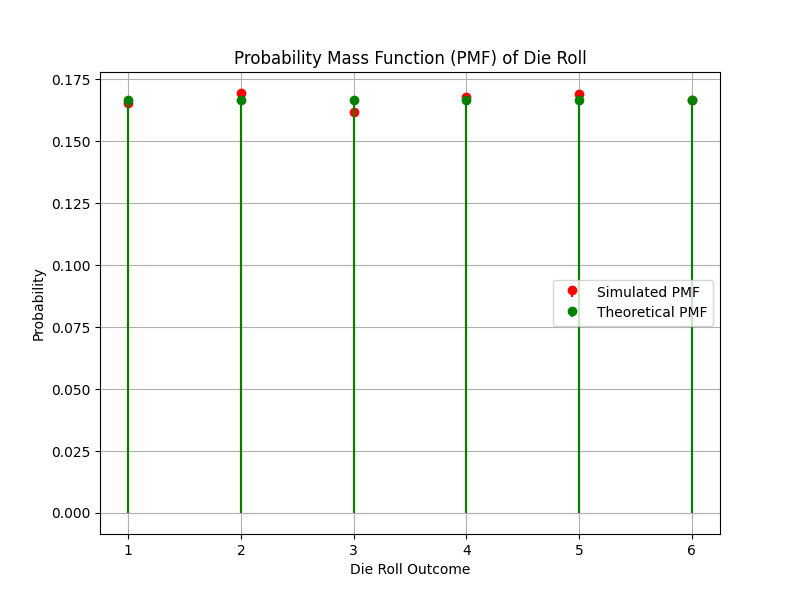
\includegraphics[width=\linewidth]{figs/Fig1.png}
		\end{figure}
	\end{frame}
	\begin{frame}
		\frametitle{Diagram}
		\begin{figure}[!ht]
			\centering
			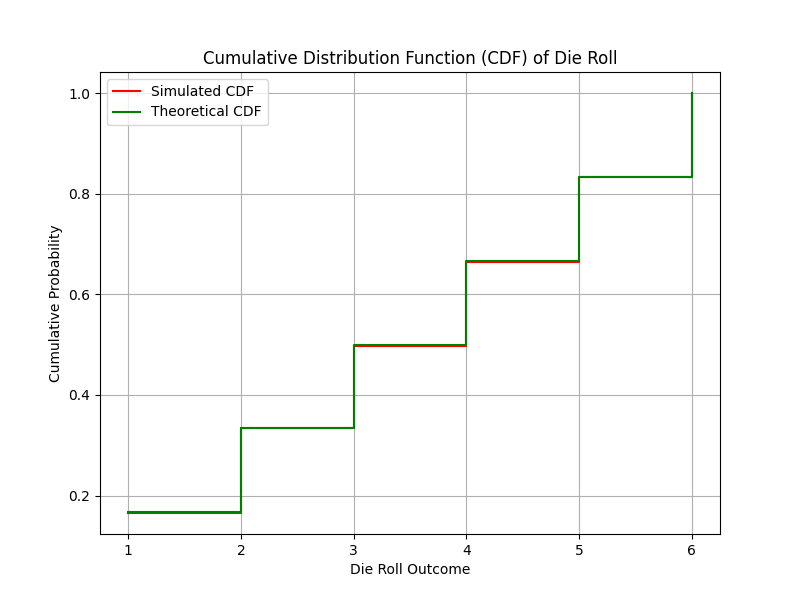
\includegraphics[width=\linewidth]{figs/Fig2.png}
		\end{figure}
	\end{frame}
\end{document}